\documentclass[12pt]{article}
\usepackage{graphicx}
\usepackage{epstopdf}         % fuer das Einbinden von Grafiken
%%\usepackage[ngerman]{babel}   % weglassen, wenn in Englisch
%% wenn Sie das ngerman package benutzen, koennen Umlaute als "a.. geschrieben
%% werden, sonst \"a..
\usepackage[latin1]{inputenc}
\usepackage{amsmath}
\usepackage{csvsimple}
\usepackage{pgfplotstable}
%% dieses package erlaubt, bei deutscher Tastatur Umlaute, � direkt einzugeben

\textwidth=170mm
\textheight=250mm
\hoffset= -20mm       % may need change
\voffset= -25mm       % may need change

%% everything after % is a comment in LATEX

\begin{document}

%% we do the title page ourselves
\thispagestyle{empty}     % only for frontpage
\null\vspace{40mm}
\begin{center}
{%%%%%%%%%%%%%%%%%%%%%%%%%% Titel
\Large  Cyclotron frequency in a Penning
trap
\footnote{\noindent Experiment F47, performed on 1.1.03,
Supervisor Patrick Wilhelm,
long special evaluation}
}\\[15mm]
%%%%%%%%%%%%%%%%%%%%%%%%%%% Authors
Thukydides Vesely, Franz Sattler

\vspace{25mm}

\parbox{0.9\textwidth}{   %% etwas schmaler als normaler Satz
Abstract:    
\small The functionality of a Penning Trap has been examined in this experiment. First, we determined the resonance Frequency of the Circuit. By exciting the oscillation modes of the trapped electrons we then determined their frequencies. Using this, as well as some other setup parameters, we were able to calculate the dimensions of the Penning trap.
}
\end{center}

\vfill
As special Evaluation attested: Date, Signature:
\vspace{20mm}

%% Rueckseite des Titelblatts leer. Bei einseitigem Druck entfernen
\newpage  
\null\thispagestyle{empty} 
   
%\newpage     % Inhaltsverzeichnis, koennte man bei langer Version machen
%\tableofcontents 

\newpage

\pagenumbering{arabic} %% start page 1 
\section{Introduction}
In this experiment we examined a penning trap. To detect the presence of electrons inside the trap, we used a multi-frequency signal sent through the Penning trap's ring electrode and varied the ring voltage which induces the vertical oscillation of the electrons. Through this method we were able to determine the resonance frequency of the circuit.
Further on we excited the modes of the electron oscillation using an antenna; which leads to a measurable drop in the amount of electrons in the trap. Using this information we can calculate first the mode frequencies and further on the dimensions of the penning trap.

\section{Theoretical Background}

\subsection{Cyclotron motion}
The Lorentz force on a particle of charge $q$ in a magnetic field $\vec{B}$ is 
\begin{equation} \vec{F}=q \vec{v} \times \vec{B} \end{equation}
Therefore, by using the centripetal Force we get for the cyclotron frequency:
\begin{equation} \omega = \frac{q}{m}B \end{equation}
Which can be used to calculate the mass of the particle, in our case of the electron.
In our setup we we superposition an electric field $\vec{E}$ with the magnetic field $\vec{B}$ which leads to multiple simultanious oscillations of the trapped electron in the Penning trap. The Electric field in our case is:
\begin{equation} \vec{E} = c\begin{pmatrix} \frac{x}{2} \\ \frac{y}{2} \\ -z \end{pmatrix} \end{equation}
The combined fields $\vec{E}$ and $\vec{B}$ result in a more complex path of the electron, consisting of a vertical oscillation with $\omega_z$, the \textbf{axial frequency}, and two oscillations in the horizontal plane, with $\omega_+$, the \textbf{reduced cyclotron frequency}, and $\omega_-$, the \textbf{magnetron frequency}.
\begin{equation} \omega_z = \sqrt{\frac{qV}{mz^2}} \label{wzfreq} \end{equation}
\begin{figure}[h]
	\centering
	\includegraphics[width=16cm,bbllx=112,bburx=447,bblly=264,bbury=582]{cyclotronmotion.JPG}
	\caption{Figure 1: Oscillation modes of the penning trap motion}
	\label{ps}
\end{figure}

\section{Experimental Setup}
Inside a vacuum tube the penning trap's electrodes are mounted. The magnetic field is generated by a coil set up around the penning trap. The electrodes inside the trap are connected to measurement electronics outside the coil, which are themselves connected to a PC, on which the data acquisition is carried out.

\begin{figure}[h]
	\centering
	\includegraphics[width=16cm,bbllx=112,bburx=447,bblly=264,bbury=582]{versuchsaufbau.JPG}
	\caption{Figure 1: Experimental setup overview}
	\label{ps}
\end{figure}

Amplification factor is 32.80 pm 0.40


\section{Execution}

\subsection{Finding the Resonance Frequency}
First off, we started by beginning to prepare for the commencing of the start of the experiment.
Using the Network Analyzer we started by finding the resonance frequeny of the RLC circuit. The Network Analyzer showed a Fourier transform of the received signal, which was very noisy; this could be fixed by turning on TG mode - in this mode, the Analyzer itself sends signals of definite frequency off into the circuit,
otherwise the electrons in the penning trap are hardly influenced by the end caps. After turning on TG mode, we saw in the amplitude versus frequency graph multiple peaks. Out of those, the deepest peak was determined to be the resonance frequency of the circuit, as the circuit has been built so that the excitation frequency of the electrons is the same as the resonance frequency:
\begin{equation*} f_{ex_1} = (48.46 \pm 0.02) \text{MHz} \end{equation*}
The manual identification of the peak lead to the error value. The other peaks were probably caused by interference from the connected devices and resulting crosstalk.
A second measurment lead to a deeper peak and therefore a better value for the excitation frequency:
\begin{equation*} f_{ex} =  f_{ex_2} = (48.549 \pm 0.02) \text{MHz} \end{equation*}

\subsection{Preparation for the Antenna Scans}
First, we set the ring voltage to $ U=(1 \pm 0.001) \text{V} $ and the coil current to $ I=(1 \pm 0.001)\text{A} $. The we varied both parameters, which led to the expected results: Increasing the current lead to a deeper dip, as the electron trajectory was more stable and more electrons could be excited by the Network Analyzer; therefore decreasing the current led to a shallower dip, as the trajectory became less stable.
Increasing the voltage led to a higher frequency peak, decreasing it to a lower one, in accordance to \eqref{wzfreq}.
We set the timings using a python file to
\begin{equation*}
t_{load} = 50 \text{ms} \qquad
t_{wait} = 20 \text{ms} \qquad
t_{excite} = 50 \text{ms} \qquad
t_{wait2} = 25 \text{ms} \qquad
t_{detect} = 100 \text{ms}
\end{equation*}

\subsection{Manual Antenna Frequency Scan}
Just like in the previous section, we set the ring voltage to $ U=(1 \pm 0.001) \text{V} $ and the coil current to $ I=(1 \pm 0.001)\text{A} $.\\
Using the antenna we coupled the modes of the electron trajectory; we varied the frequency of the antenna manually over the whole range of the device, and found multiple positions in which the dip flattened or disappeared. This indicated that within those frequencies an energy transfer occured between the modes of the electron trajectory. As the frequencies at which this occurs should be sums or differences of the mode frequencies themselves, we could assign the corresponding modes to the transfer frequencies.
\begin{equation*}
\begin{aligned}
f_0 = 64.25 \text{MHz} \cong (\omega_z - \omega_-) \qquad f_1 = 72.8 \text{MHz} \cong \omega_z \\
f_2 = 81.06 \text{MHz} \cong (\omega_z + \omega_-)\qquad f_3 = 146.00 \text{MHz} \cong 2\omega_z
\end{aligned}
\end{equation*}
As those values were determined simply by observing the Analyzer Graph, the error of those values should be rather big. A more precise approach would be of course to record the depth of the dip and evaluate it later, as we will did in the following section.

\subsection{Rough Scripted Antenna Frequency Scan}
Using a python script we made two automated scans with the antenna over the spectrum of 
$ f \in \{ f \in [40\text{MHz},100\text{MHz}) | f \bmod 0.5 = 0\} $.
Both with a coil current of $ I=(1 \pm 0.001)\text{A} $, and one with a Voltage of $ U_1=(1 \pm 0.001) \text{V} $ and one with $ U_2=(1 \pm 0.001) \text{V} $.
The resulting graphs can be seen in Figures \eqref{fig::RFS08} and \eqref{fig::RFS10}.

\begin{figure}[h]
  \centering
  \parbox{70mm}{
    \centering
    \includegraphics[width=85mm]{08V.eps}
    \caption{Rough Frequency Scan with $0.8$V}
    \label{fig::RFS08}
  }
  \hfill
  \parbox{70mm}{
    \centering
    \includegraphics[width=85mm]{10V.eps}
    \caption{Rough Frequency Scan with $1.0$V}
    \label{fig::RFS10}
  }
\end{figure}

\subsection{Fine Scripted Antenna Frequency Scan}
Using a python script we made multiple scans with the antenna over the spectrum of 
$ f \in \{ f \in [0\text{MHz},350\text{MHz}) | f \bmod 0.1 = 0\} $. \\
One measurment series has been performed with a constant current of $ I=(1 \pm 0.001)\text{A} $ and varying voltage 
$ U \in \{ U \in [0.7\text{V},1.5\text{V}] | U \bmod 0.1 = 0\} $. \\
A second one has been performed with a constant voltage of $ U=(1 \pm 0.001)\text{V} $ and varying current
$ I \in \{ I \in [0.7\text{A},1.3\text{A}] | I \bmod 0.1 = 0\} $.\\
The resulting graphs can be seen in Figure \eqref{fig::FFS}.

\begin{figure}[h]
	\centering
	\includegraphics[width=16cm,bbllx=112,bburx=447,bblly=264,bbury=582]{versuchsaufbau.JPG}
	\caption{Fine Frequency Scan}
	\label{fig::FFS}
\end{figure}

\subsection{Determination of the Electron Lifetime}
placeholder

\section{Evaluation of Results}
\subsection{Coil Parameters}
For later calculations we will need coil inductivity $L$, which we can obtain from the coil parameters $n$, the amount of windings throughout one cm, and the length $l$ of the coil.
The winding number can be determined through two means: $n_1$ was found through counting the windings through one cm, $n_2$ by measuring the thickness of the wire and dividing 1cm through it.
\begin{equation*}
\begin{aligned}
l = (24.5 \pm 0.2)cm \\
d = 0.85mm \\
n_1 = 295 \\
n_2 = 288
\end{aligned}
\end{equation*}
Now we can calculate $n$ by taking the mean of $n_1$ and $n_2$ and we estimate an error:
\begin{equation*}
n = (292 \pm 5)
\end{equation*}
Therefore, the inductivity of the coil is
\begin{equation*}
L = \mu_0\frac{n}{l} = (1.50 \pm 0.03)\frac{mT}{A}
\end{equation*}

\subsection{Voltage Scan}

\begin{figure}[h]
  \centering
  \includegraphics[width=20cm,bbllx=112,bburx=447,bblly=264,bbury=582]{Graph3.eps}
  \caption{Frequency vs Voltage of mode Energy Transfer}
  \label{fig::dips}
\end{figure}

First off, we determined the positions of the dips in Figure \eqref{fig::dips} and documented their frequency values in Table 1. The multiples of $\omega_z$ are the deepest dips in the figure; for each configuration of Voltage and Current the mean of the multiples has been taken. Around those there are always two equidistant dips whose frequencies are determined through $(\omega_z \pm \omega_-)$, thus those give us values for $\omega_-$ which means are documented in Table 1 for each configuration.
The lonely dip at the end of the spectrum represents $\omega_+$, which is also documented in Table 1.

\pgfplotstabletypeset[
    col sep=comma,
    string type,
    every head row/.style={%
        before row={\hline
            \multicolumn{7}{c}{\textbf{Table 1: Frequencies for voltage variable}} & \\
        },
        after row=\hline
    },
    every last row/.style={after row=\hline},
    columns/V/.style={column name=Voltage, column type=c},
    columns/dV/.style={column name=Error, column type=c},
    columns/wz/.style={column name=$\omega_z$, column type=c},
    columns/dwz/.style={column name=$\Delta\omega_z$, column type=c},
    columns/wm/.style={column name=$\omega_-$, column type=c},
    columns/dwm/.style={column name=$\Delta\omega_-$, column type=c},
    columns/wp/.style={column name=$\omega_+$, column type=c},
    columns/dwp/.style={column name=$\Delta\omega_+$, column type=c}
    ]{tableVarVoltage.csv}

The values of Table 1 are plotted below in Figure \eqref{fig::varVolt}. We observe an obvious dependence of $\omega_z$ from the Voltage. As seen in the theoretical Section, it holds that:

\begin{equation*}
\begin{aligned}
\omega_z = \sqrt{\frac{q}{m z_0^2}V} = \sqrt{A V} \\
\Rightarrow z_0 = \sqrt{\frac{q}{m A}}
\end{aligned}
\end{equation*}

The above dependence between $\omega_z$ and $V$ has been fitted to the data in Figure \eqref{fig::varVolt}.

\begin{figure}[h]
  \centering
  \includegraphics[width=20cm,bbllx=112,bburx=447,bblly=264,bbury=582]{Graph3.eps}
  \caption{Frequency vs Voltage of mode Energy Transfer}
  \label{fig::varVolt}
\end{figure}

Using the above equation, as well as the electron mass $m = 9.108*10^{-31} \text{kg}$ and the elementary electron charge $q = 1.602*10^{-19}\text{C}$, we obtain the Penning trap electrode width through using the result $A = (161.3 \pm 1.1) \frac{\text{MHz}^2}{\text{V}}$:

\begin{equation*}
\begin{aligned}
z_0 = (3.302 \pm 0.001) \text{cm} \\
\Rightarrow \rho_0 = \sqrt{2}z_0 = (4.670 \pm 0.001) \text{cm}
\end{aligned}
\end{equation*} 

Especially the above dependence between $\omega_z$ and the voltage can be seen as confirmed, because the relative error for A is as small as 0.66\%.

\subsection{Current Scan}

The dips here have been evaluated in the same way as in the subsection above. The results can be seen in Table 2:

\pgfplotstabletypeset[
    col sep=comma,
    string type,
    every head row/.style={%
        before row={\hline
            \multicolumn{6}{c}{\textbf{Table 2: Frequencies for current variable}} & \\
        },
        after row=\hline
    },
    every last row/.style={after row=\hline},
    columns/I/.style={column name=Current, column type=c},
    columns/wz/.style={column name=$\omega_z$, column type=c},
    columns/dwz/.style={column name=$\Delta\omega_z$, column type=c},
    columns/wm/.style={column name=$\omega_-$, column type=c},
    columns/dwm/.style={column name=$\Delta\omega_-$, column type=c},
    columns/wp/.style={column name=$\omega_+$, column type=c},
    columns/dwp/.style={column name=$\Delta\omega_+$, column type=c}
    ]{tableVarCurrent.csv}

The values of Table 2 are plotted below in Figure \eqref{fig::varCur}. We observe an obvious dependence of $\omega_-$ from the Current. As seen in the theoretical Section, it holds that:

\begin{equation*}
\begin{aligned}
\omega_- = \frac{1}{2}(\omega_c - \sqrt{\omega_c^2 - 2\omega_z^2}) \\
\omega_c = \frac{q}{m}B \\
\omega_z = (73.35 \pm 0.28) \text{MHz}
\end{aligned}
\end{equation*}

The above dependence between $\omega_-$ and $V$ has been fitted to the data in Figure \eqref{fig::varCur}.

\begin{figure}[h]
  \centering
  \includegraphics[width=20cm,bbllx=112,bburx=447,bblly=264,bbury=582]{Graph4.eps}
  \caption{Frequency vs current of mode Energy Transfer}
  \label{fig::varCur}
\end{figure}

Through the fit we obtain the electron mass as $m = (7.490 \pm 0.085)*10^{-31}\text{kg}$. The literature value is $(9.10938356 \pm 0.00000011)*10^{-31}\text{kg}$\cite{cod}, which is about 20 standard deviations away from our value.
It seems like a systematic error through which the frequency falls too fast with the current.
The discrepancy could be also partially attributed to the hardly discernible dips for higher Currents (as the noise increases drastically) as well as for lower Currents (as the electron trajectory becomes less stable).
The small error seems to be a coincidence.
\section{Discussion}

\newpage 
%% hier wird 'von Hand' eine neue Seite erzwungen

%% Literatur)

\begin{thebibliography}{00}   % {00}: max 2-stellige Referenznummer

\bibitem{cod} 2014 CODATA
\bibitem{uwe} Uwe Ludwig, private Mitteilung
\bibitem{karl} Karl Popper, Phys.~Rev.~Lett.~95 (2001) 25
\bibitem{dipl} K. Winter, Diplomarbeit Heidelberg (1968)
\bibitem{bibel} Genesis 3,4

\end{thebibliography}

\end{document}
